\subsubsection{Modelo communication health services}
\label{modelo_communication_health_services}

Un sistema \gls{iot} necesita de un buen sistema de monitorización y comunicación de su estado actual de salud, comúnmente llamado \gls{housekeeping}. Podemos evitar posibles problemas en el dispositivo si contamos con la información necesaria.

Para ello, utilizaremos una monitorización constante de variables del sistema tales como cargas de CPU, memoria, tráfico de red, estado de las particiones de disco.
Modelamos el sistema utilizando el modelo \textit{HealthMonitor} el cual define una entidad abstracta de monitorización de salud.

\begin{figure}[ht]
	\centering
    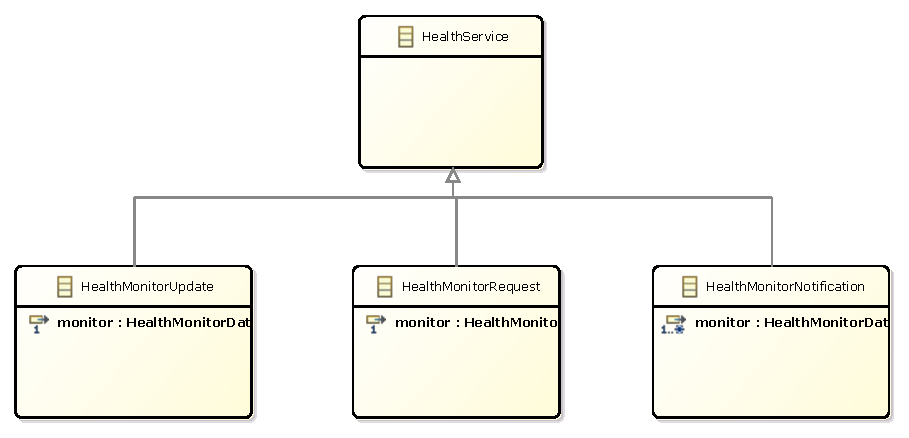
\includegraphics[height=0.3\textheight]{images/models/communicationshealths_class_diagram.pdf}
    \captionmodeloclase{Servicios comunicación - Housekeeping (Estado de salud).}
    \label{fig:modelo_servicios_comunicacion_health_classes}
\end{figure}

Para la comunicación del estado de salud definimos el servicio \textit{HealthService} y dos subservicios tal como puede verse en la figura \ref{fig:modelo_servicios_comunicacion_health_classes}: \textit{MonitorItems} y \textit{MonitorChangeItemInterval}, primer servicio utilizado para enviar el estado de todos los sensores activos desde el dispositivo \gls{iot} al servidor.

El segundo subservicio lo utilizaremos para modificar el intervalo de captura del estado de salud de un elemento en concreto, pudiendo especificar si se desea recuperar la información actual sin esperar al intervalo de tiempo del elemento a monitorizar.

Este modelo necesita de los datos proporcionados el modelo salud en la sección \ref{modelo_health}.
